
\noindent\textbf{8. (CRLS 22.3-2)} Mostre como a \proc{DFS} funciona no grafo da Figura 22.6 do CLRS (segunda
edição). Assuma que o laço das linhas 5-7 da \proc{DFS} visitam os vértices em ordem alfabética, e que
os vértices se encontram em ordem alfabética nas listas de adjacências. Mostre os valores de $d$ e $f$
para cada vértice ao final da \proc{DFS}.

\textbf{Resposta:} A figura \ref{fig:7.8-1} mostra o rastreamento da \proc{DFS} em 3 momentos distintos: quando todos os vértices adjacentes à $w$ são visitados, todos os vértices adjacentes à $t$ são visitados e a árvore com todas as chamadas recursivas concluídas, respectivamente.

Os valores $d$ e $f$, bem como o antecessor de cada vértice dado por $\pi$ estão na tabela de rastreamento abaixo de cada imagem. Os tipos de arestas também estão devidamente destacados.

\begin{center}
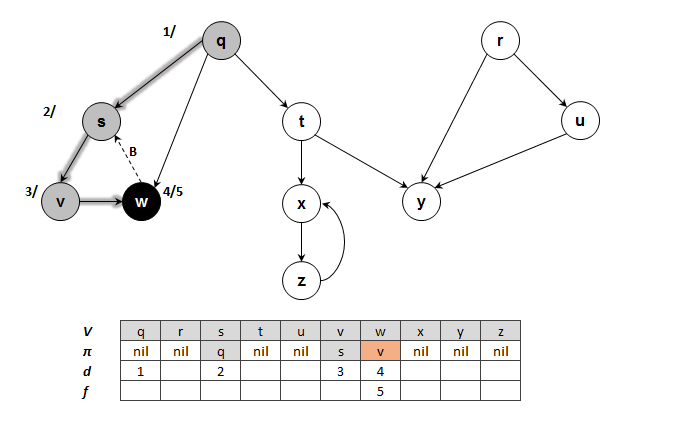
\includegraphics[width=0.9\textwidth]{q7-08-p1.png}
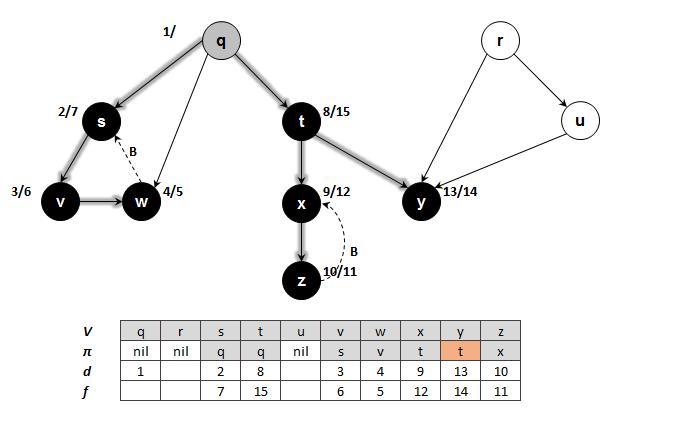
\includegraphics[width=0.9\textwidth]{q7-08-p2.png}
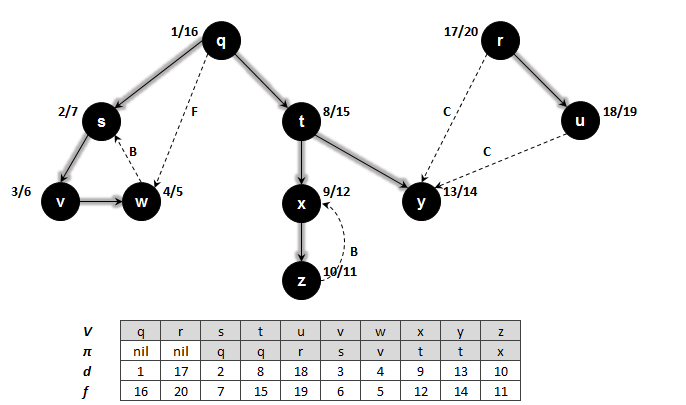
\includegraphics[width=0.9\textwidth]{q7-08-p3.png}
\captionof{figure}{Rastreamento da \proc{DFS} na figura 22.6 do CLRS.}
\label{fig:7.8-1}
\end{center}